\renewcommand{\tmpwidth}{32mm}
\setlength{\tabcolsep}{2pt}
\begin{figure*}[!ht]
    \centering
    %\renewcommand{\arraystretch}{2}
    \begin{tabular}{cc}
% \includegraphics[ height=\tmpwidth]{figures/panorama/000020_ours.jpeg} \\ 
Input & \model (Ours)
\\ 

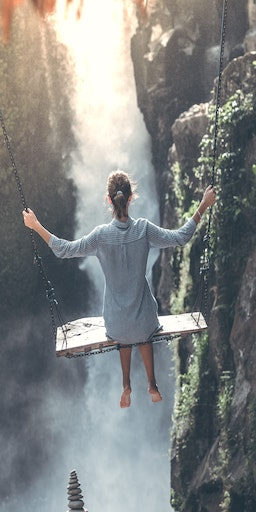
\includegraphics[ height=\tmpwidth]{figures/panorama/artem-beliaikin-8AsKha7aIvk-unsplash.jpg} &
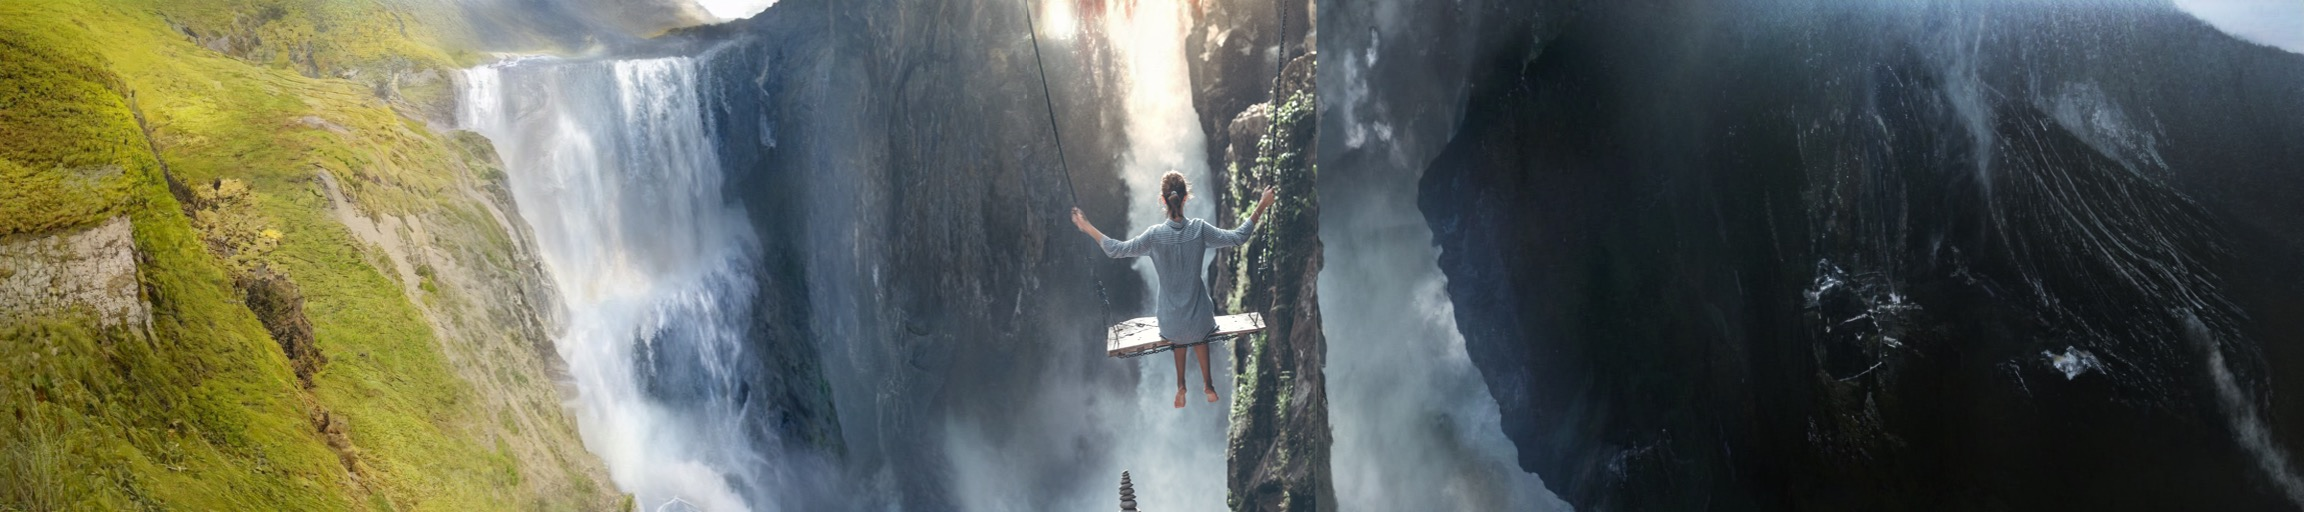
\includegraphics[ height=\tmpwidth]{figures/panorama/artem-beliaikin-8AsKha7aIvk-unsplash_ours.jpeg} \\ 


% \includegraphics[ height=\tmpwidth]{figures/panorama/damiano-baschiera-hFXZ5cNfkOk-unsplash.jpg_input.jpeg} \\ 
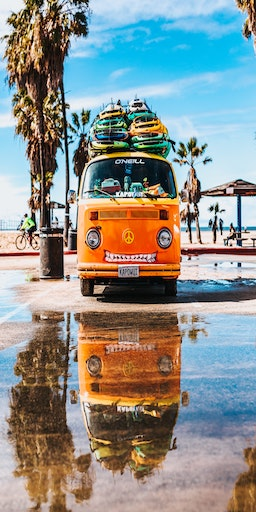
\includegraphics[ height=\tmpwidth]{figures/panorama/tyler-nix-6mze64HRU2Q-unsplash.jpg} &
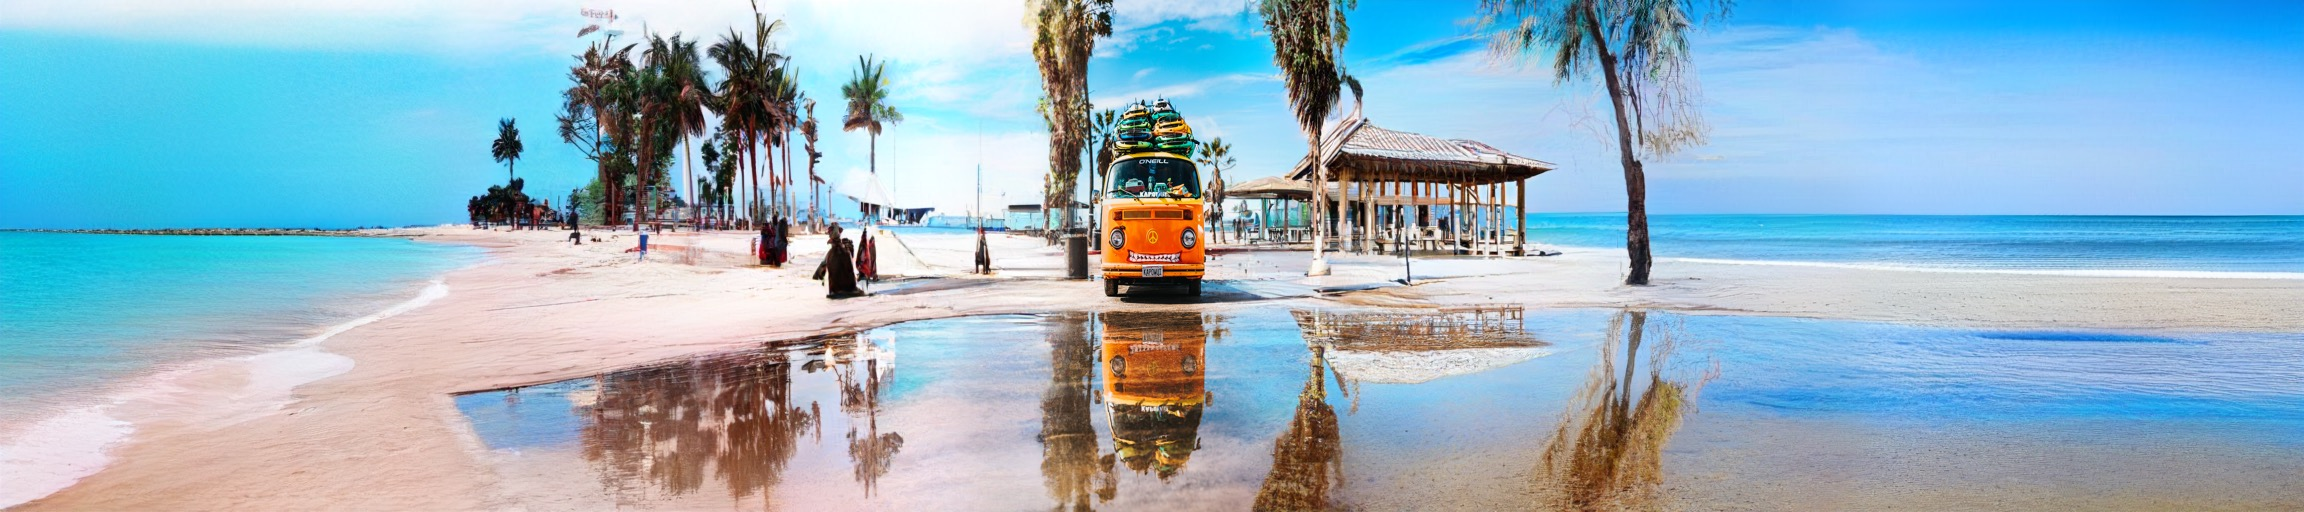
\includegraphics[ height=\tmpwidth]{figures/panorama/tyler-nix-6mze64HRU2Q-unsplash_panorama.jpeg} \\ 
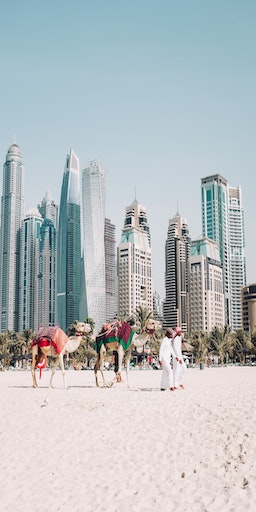
\includegraphics[ height=\tmpwidth]{figures/panorama/fredrik-ohlander-fCW1hWq2nq0-unsplash.jpg} &
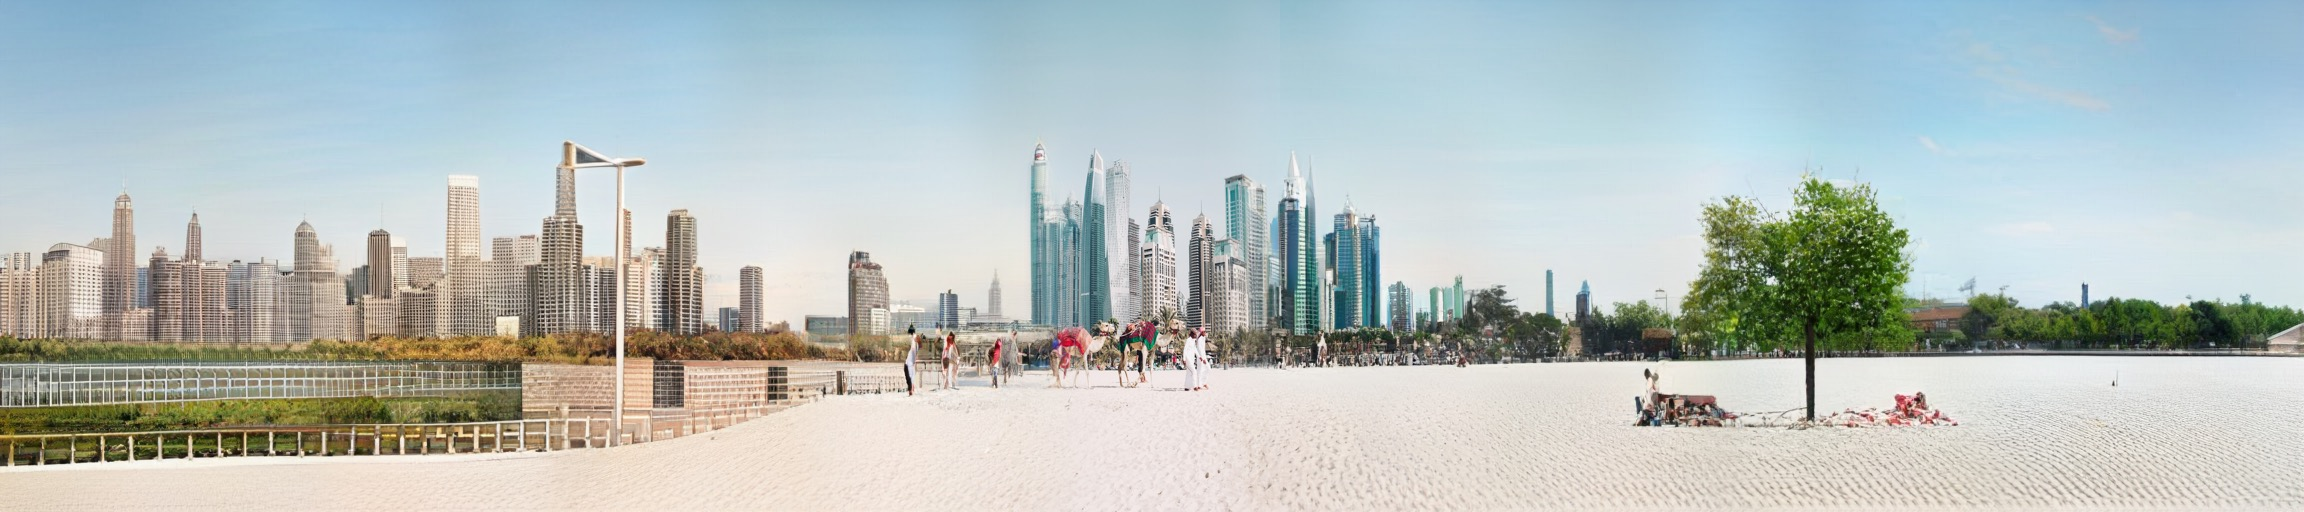
\includegraphics[ height=\tmpwidth]{figures/panorama/fredrik-ohlander-fCW1hWq2nq0-unsplash.jpg_input.jpeg} \\ 

% \includegraphics[ height=\tmpwidth]{figures/panorama/jairph-1XLyzi17Z2M-unsplash.jpg_input.jpeg} \\ 
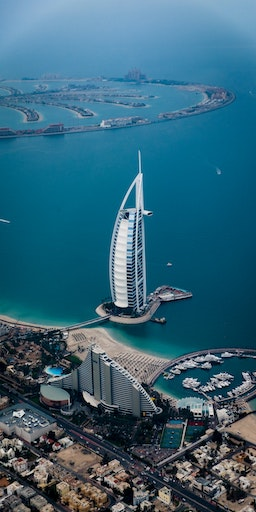
\includegraphics[ height=\tmpwidth]{figures/panorama/christoph-schulz-7tb-b37yHx4-unsplash.jpg} &
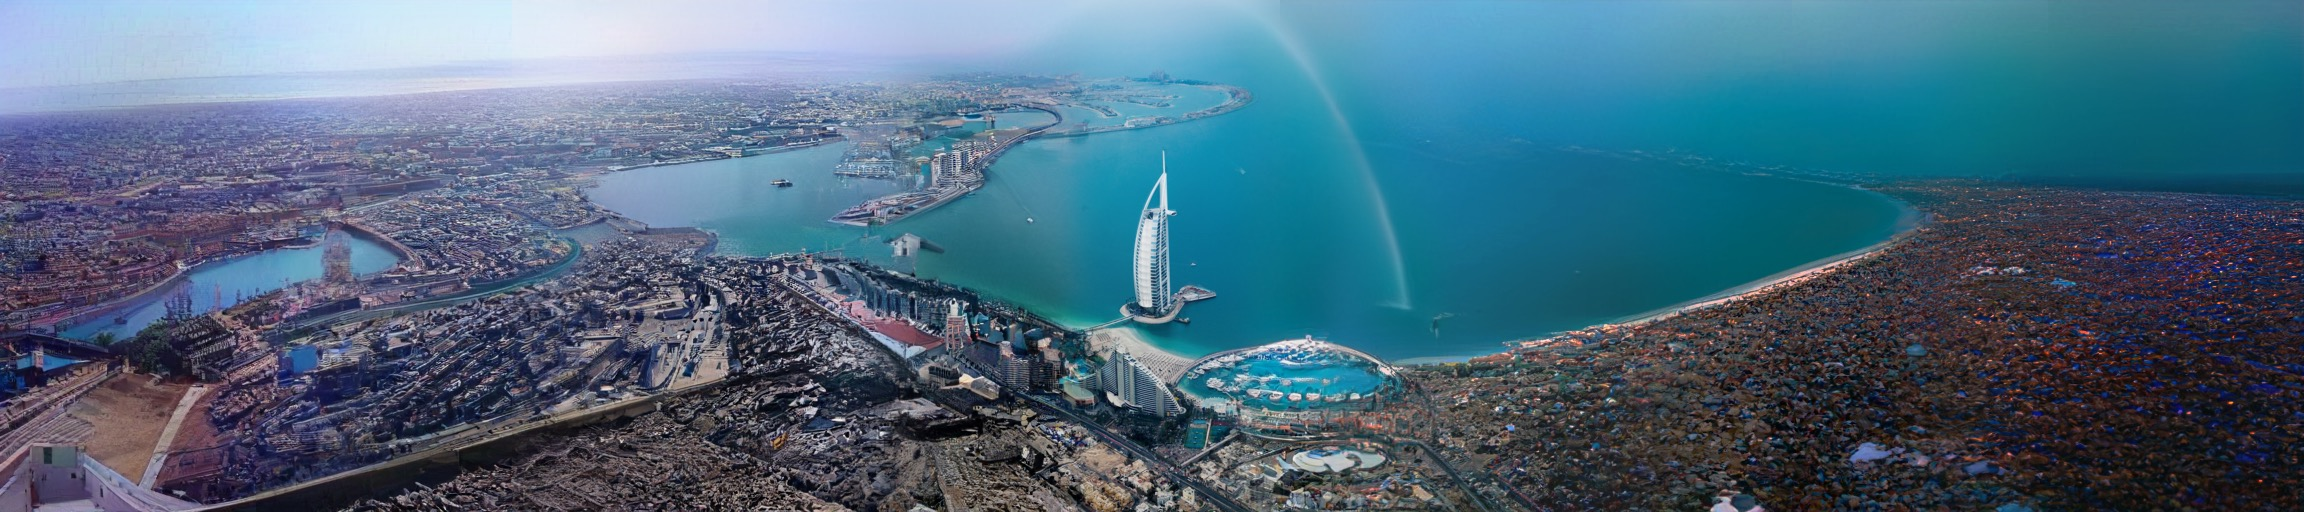
\includegraphics[ height=\tmpwidth]{figures/panorama/christoph-schulz-7tb-b37yHx4-unsplash.jpg_input.jpeg} \\ 
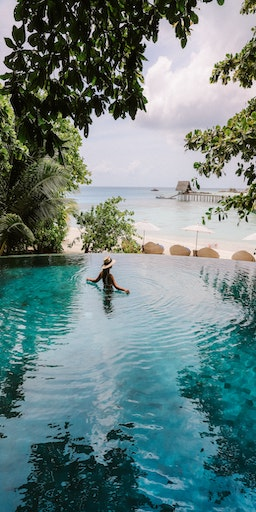
\includegraphics[ height=\tmpwidth]{figures/panorama/chelsea-gates-0653_wY0nRc-unsplash.jpg} &
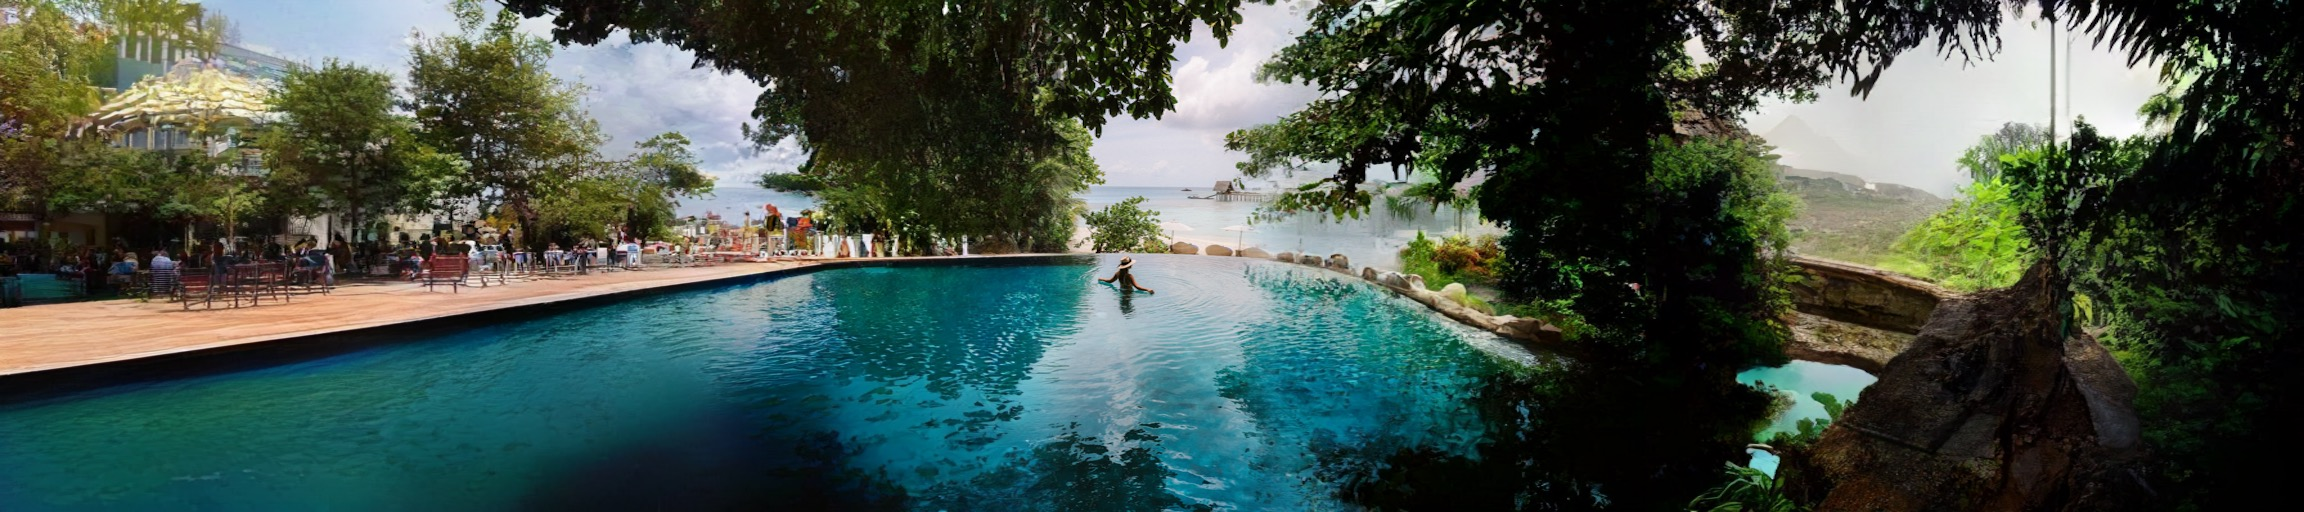
\includegraphics[ height=\tmpwidth]{figures/panorama/chelsea-gates-0653_wY0nRc-unsplash.jpg_input.jpeg} \\ 
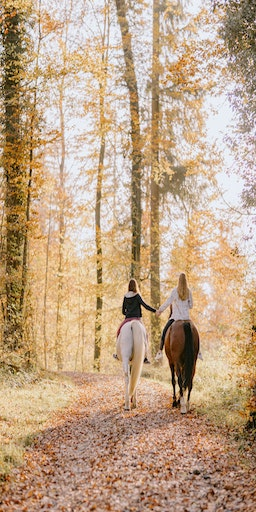
\includegraphics[ height=\tmpwidth]{figures/panorama/janosch-diggelmann-qXzNdOfGnbw-unsplash.jpg} &
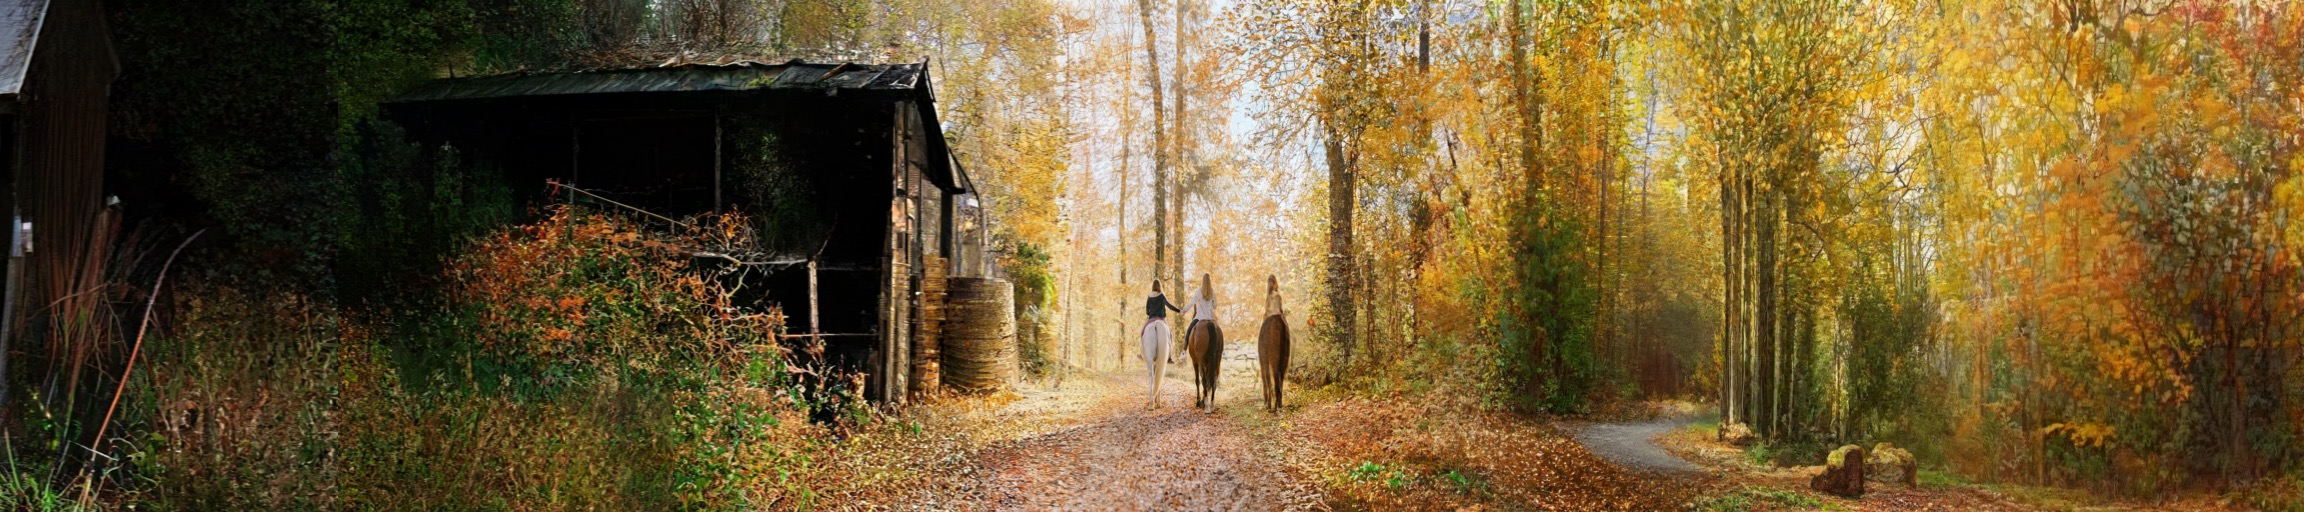
\includegraphics[ height=\tmpwidth]{figures/panorama/janosch-diggelmann-qXzNdOfGnbw-unsplash2.jpg_input.jpeg} \\ 

    \end{tabular}
    \vspace{-3mm}
    \caption{More Samples of Horizontal Image Extrapolation (from 512$\times$256 to 512$\times$2304). The synthesized "panoramas" are created by repeatedly applying \model's outpainting abilities horizontally in both directions.}
    %\vspace{-6mm}
    \label{fig:supp_panorama}
\end{figure*}

